\titleframe

% -----------------------------------------------------------------------------
% Slide 2: Motivation of Today
% -----------------------------------------------------------------------------
\begin{frame}{Motivation of Today}
  \framesubtitle{Room 0/64, Building B37, Educational Microgrid Setup}
  \begin{center}
    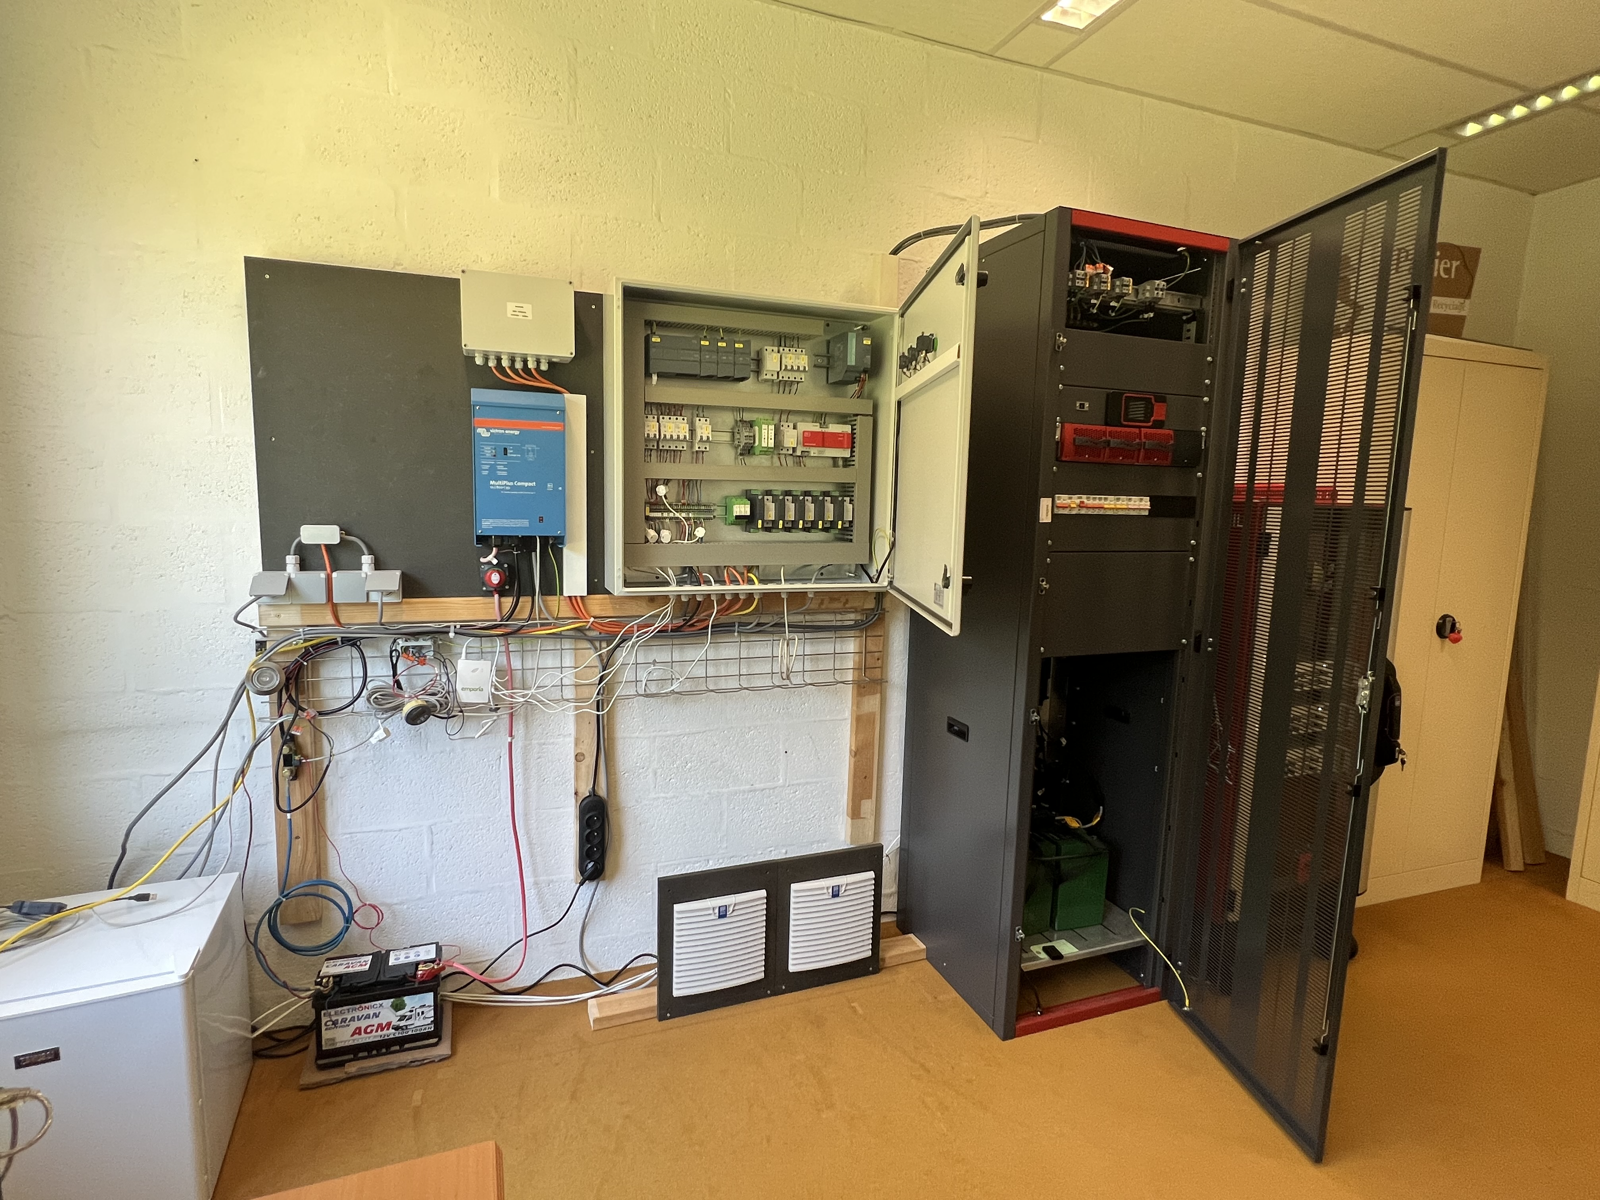
\includegraphics[width=0.88\textwidth,height=0.68\textheight,keepaspectratio]{images/room_b37.png}
  \end{center}
\end{frame}

% -----------------------------------------------------------------------------
% Slide 3: Motivation of Today - Single-Wire Diagram
% -----------------------------------------------------------------------------
\begin{frame}{Motivation of Today}
  \framesubtitle{Single-Wire Equivalent Diagram: How do these devices work?}
  \begin{center}
    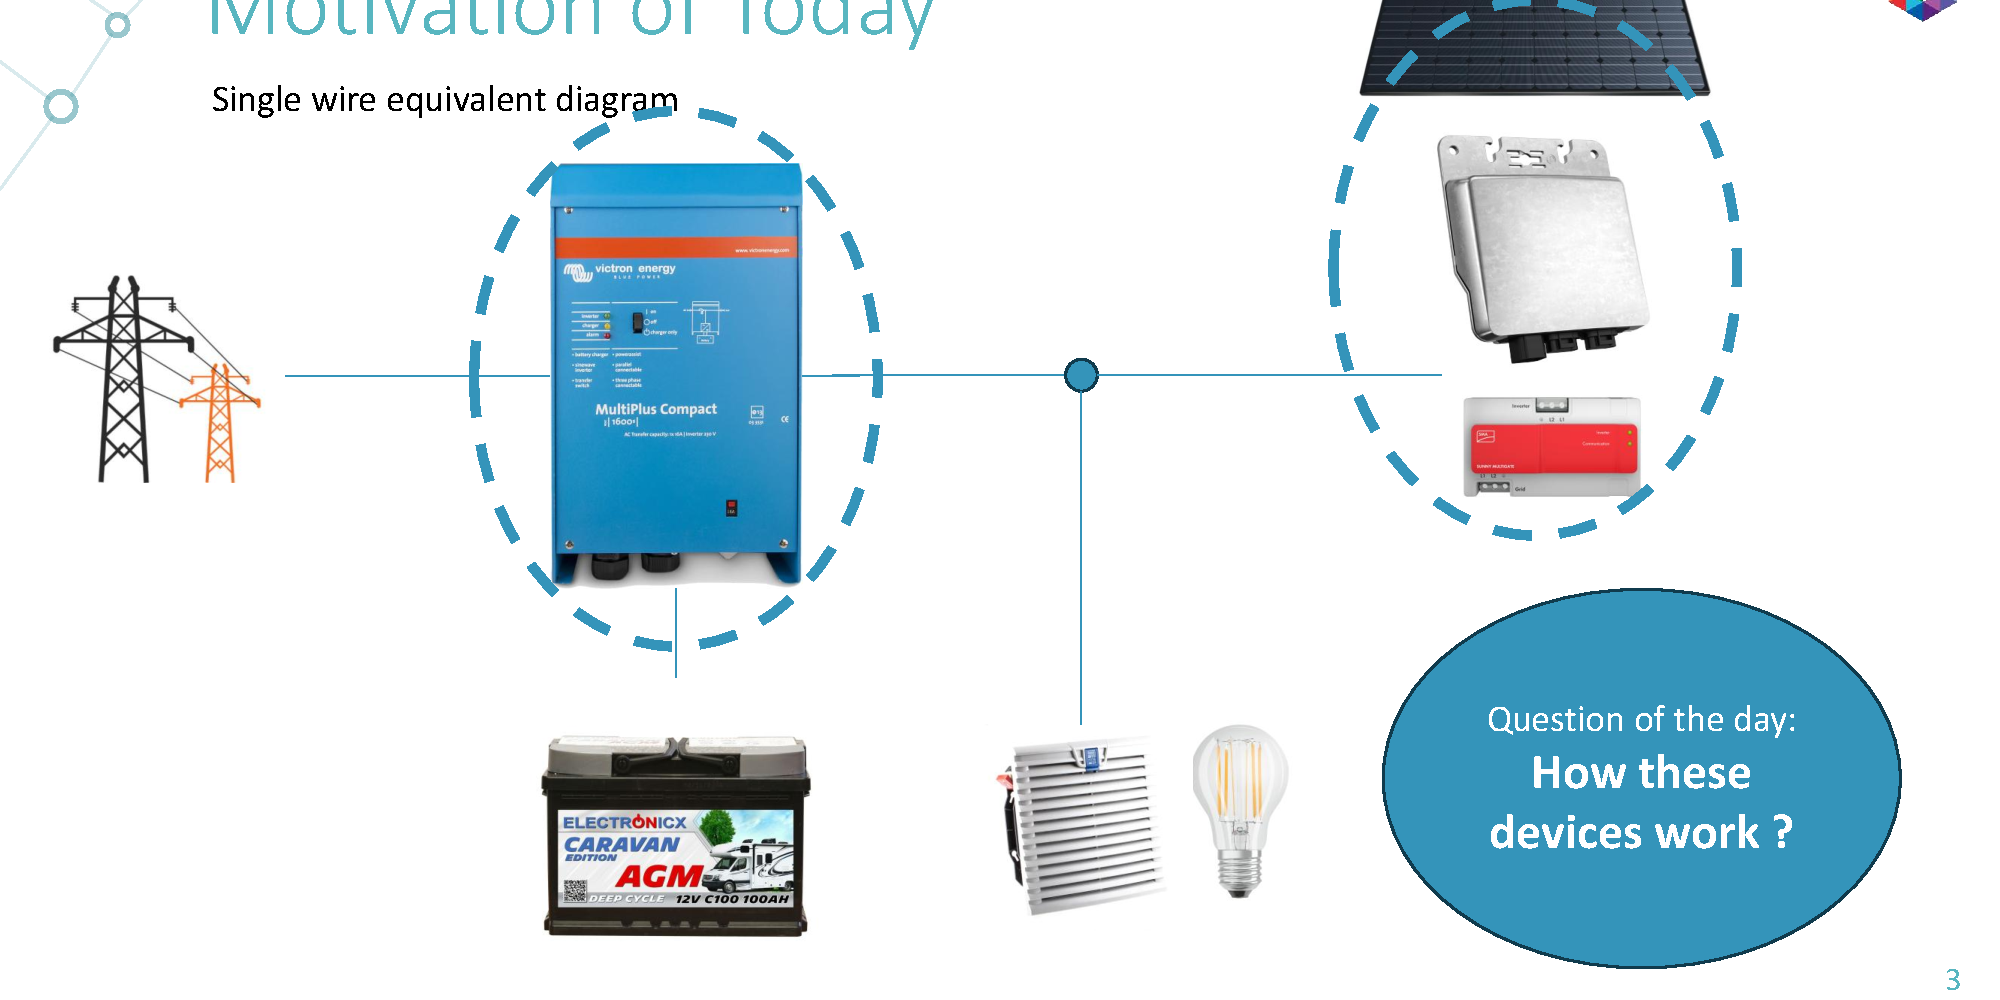
\includegraphics[width=0.90\textwidth,height=0.68\textheight,keepaspectratio]{images/single_wire_b37.pdf}
  \end{center}
\end{frame}

% -----------------------------------------------------------------------------
% Slide 4: Outline
% -----------------------------------------------------------------------------
\begin{frame}{Outline}
  \tableofcontents
\end{frame}

% =============================================================================
% SECTION 1: Voltage Source Converter (VSC)
% =============================================================================
\section{Voltage Source Converter (VSC)}

% -----------------------------------------------------------------------------
% Slide 6: Classification of Converters
% -----------------------------------------------------------------------------
\begin{frame}{Classification of Converters}
  \framesubtitle{According to Mohan et al. and Yazdani \& Iravani [1, 2]}
  \begin{center}
    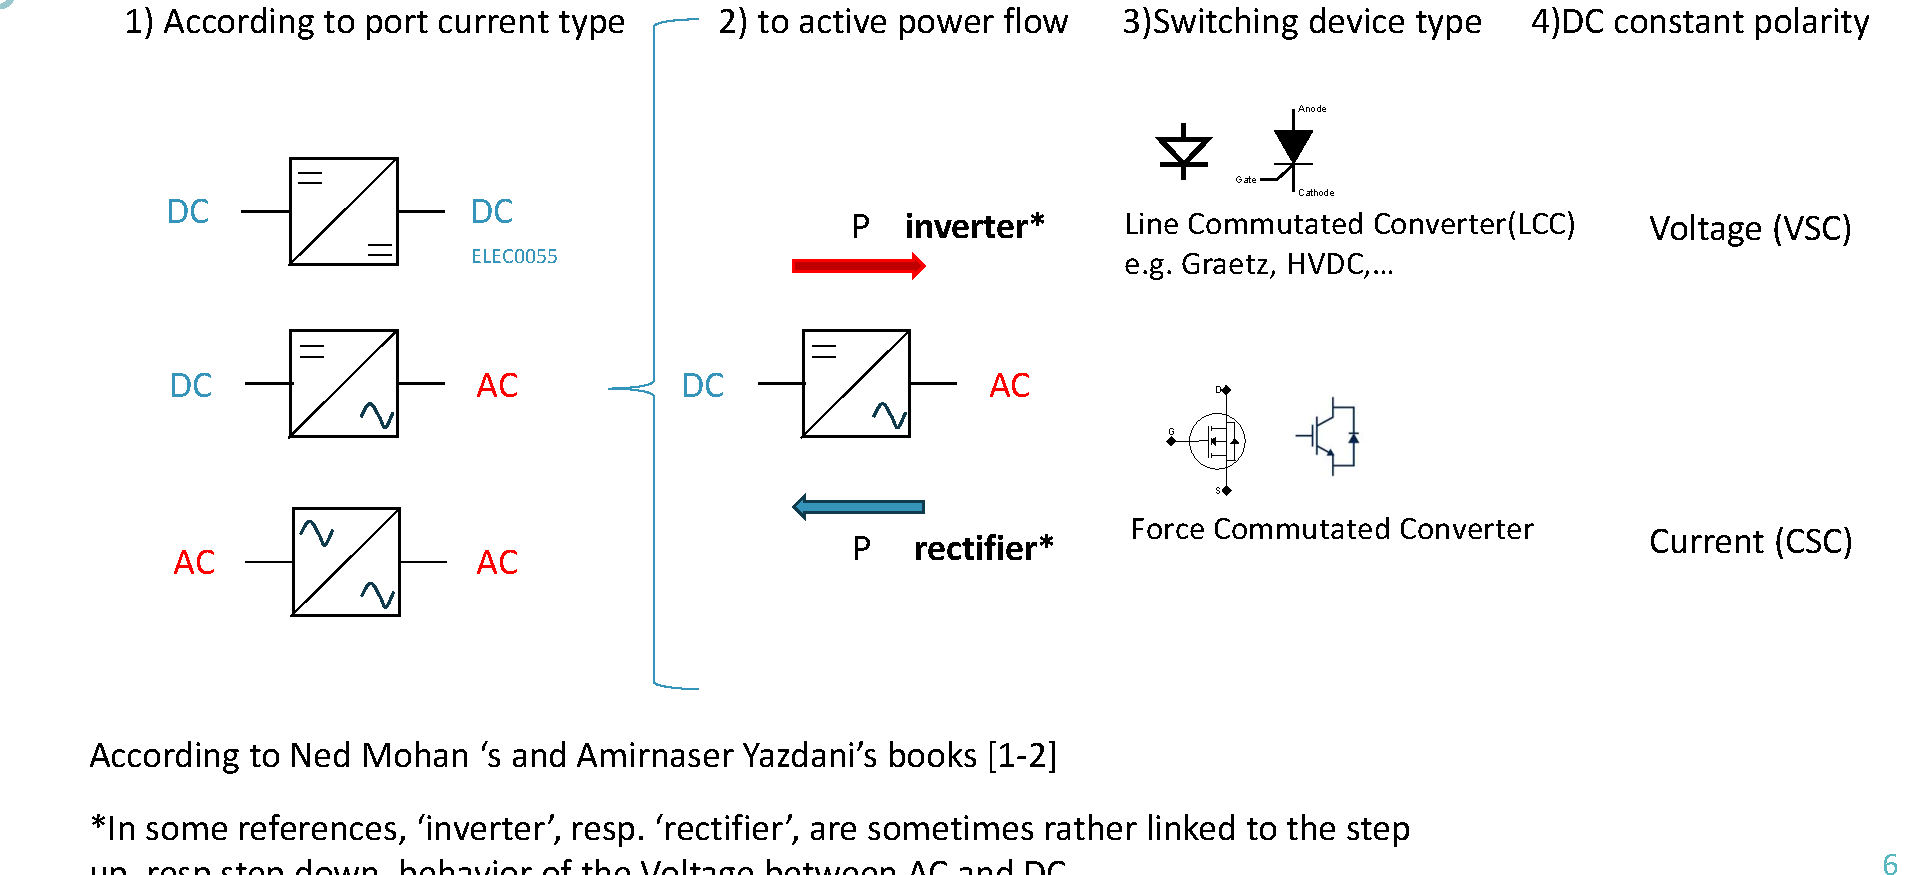
\includegraphics[width=0.90\textwidth,height=0.68\textheight,keepaspectratio]{images/classification_converters_1.pdf}
  \end{center}
\end{frame}

% -----------------------------------------------------------------------------
% Slide 7: How Would You Classify Our Devices?
% -----------------------------------------------------------------------------
\begin{frame}{How Would You Classify Our Devices?}
  \begin{center}
    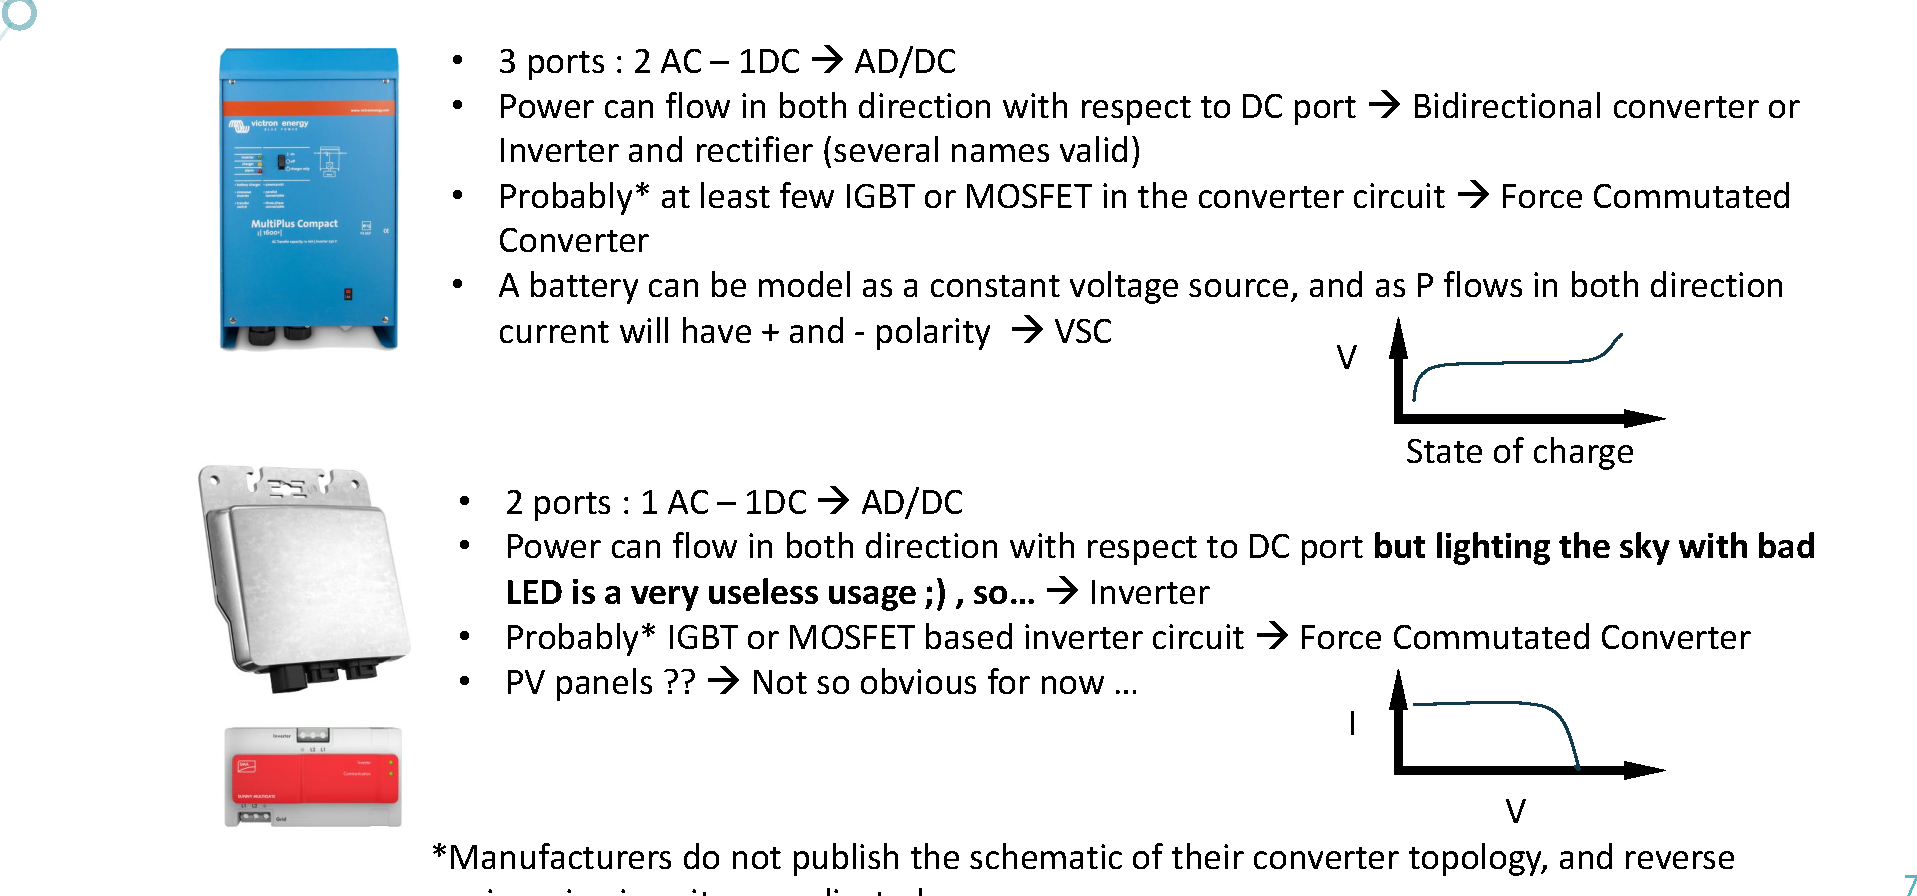
\includegraphics[width=0.90\textwidth,height=0.68\textheight,keepaspectratio]{images/device_classification.pdf}
  \end{center}
\end{frame}

% -----------------------------------------------------------------------------
% Slide 8: Classification of Converters - Focus on VSC
% -----------------------------------------------------------------------------
\begin{frame}{Classification of Converters: Focus on VSC}
  \framesubtitle{Forced commutated voltage source converters (Scope of today)}
  \begin{center}
    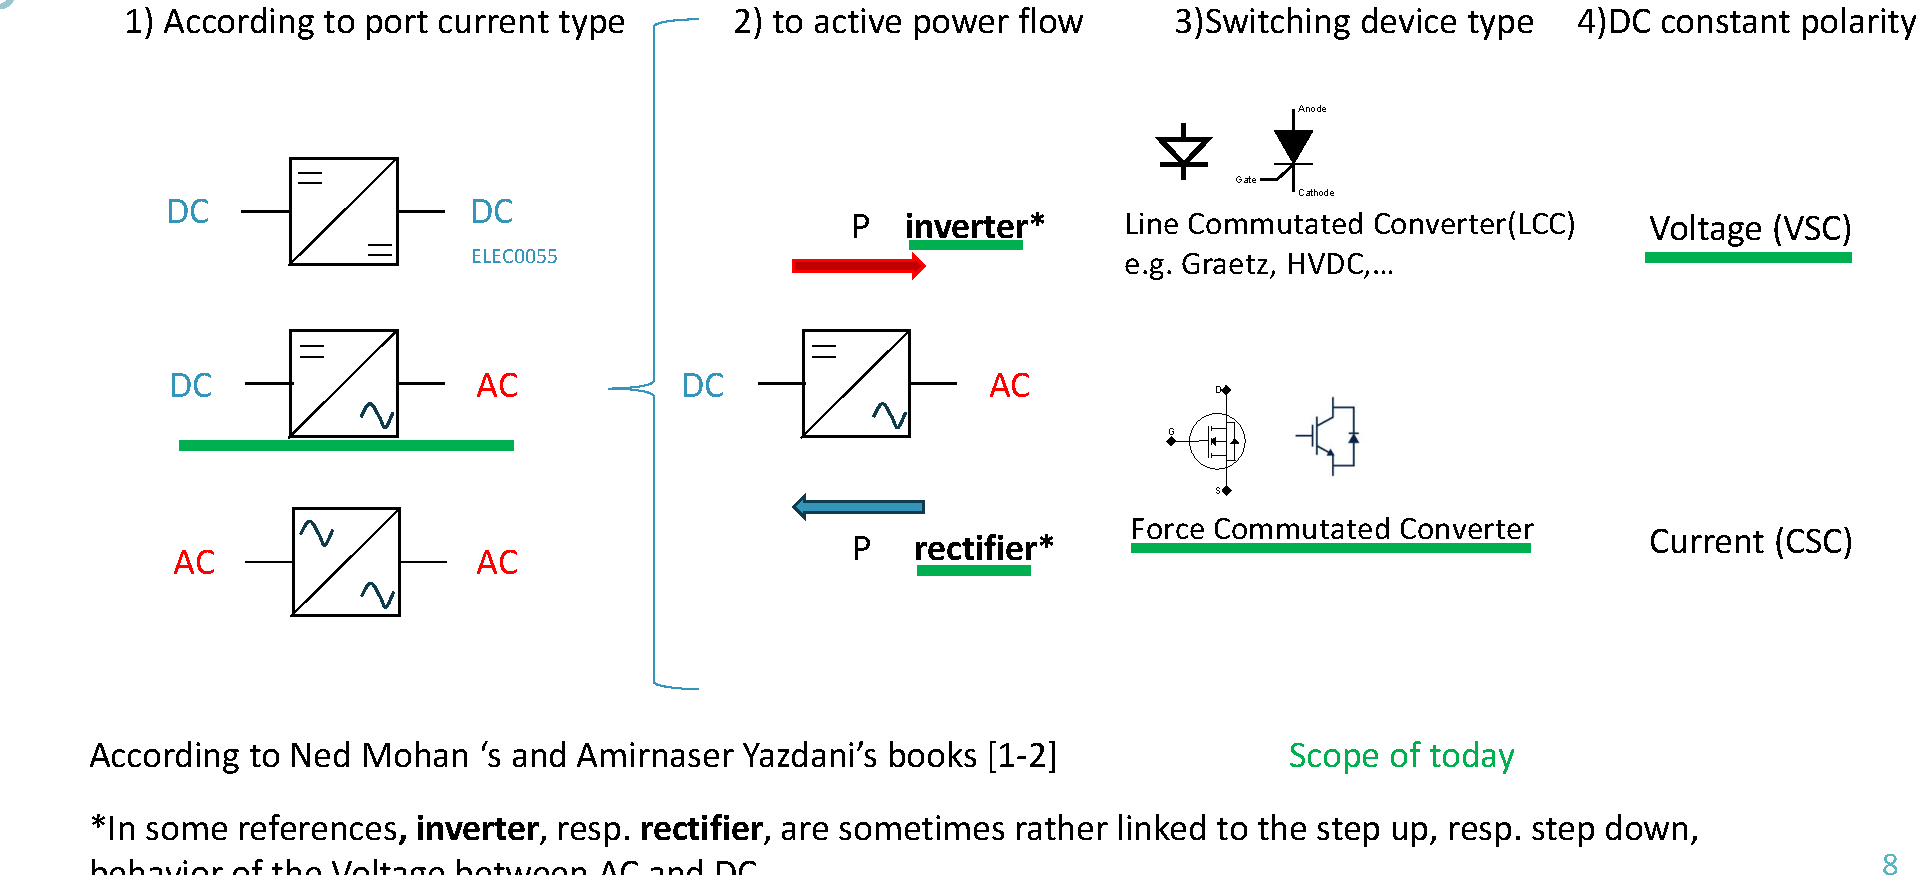
\includegraphics[width=0.90\textwidth,height=0.68\textheight,keepaspectratio]{images/classification_converters_2.pdf}
  \end{center}
\end{frame}

% -----------------------------------------------------------------------------
% Slide 9: AC-DC Topology in Practice
% -----------------------------------------------------------------------------
\begin{frame}{AC-DC Topologies in Practice}
  \vspace{-0.5em}
  \begin{columns}[T]
    \begin{column}{0.31\textwidth}
      \centering
      \textbf{Half-Bridge ($1\phi$)}\\[0.2em]
      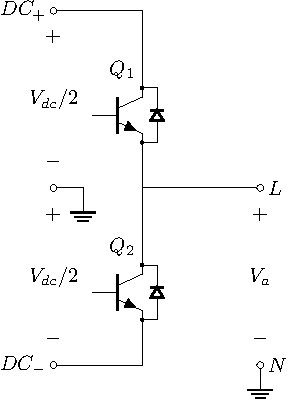
\includegraphics[width=0.9\textwidth,height=0.36\textheight,keepaspectratio]{half_bridge.pdf}\\[0.2em]
      {\footnotesize 2 switches\\Requires split DC bus}
    \end{column}
    \begin{column}{0.34\textwidth}
      \centering
      \textbf{Full-Bridge ($1\phi$)}\\[0.2em]
      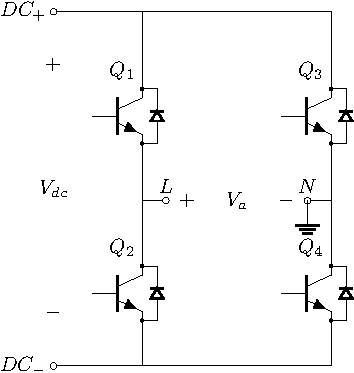
\includegraphics[width=0.9\textwidth,height=0.36\textheight,keepaspectratio]{full_bridge.pdf}\\[0.2em]
      {\footnotesize 4 switches (H-bridge)\\Bipolar / unipolar PWM}
    \end{column}
    \begin{column}{0.34\textwidth}
      \centering
      \textbf{Three-Phase Bridge ($3\phi$)}\\[0.2em]
      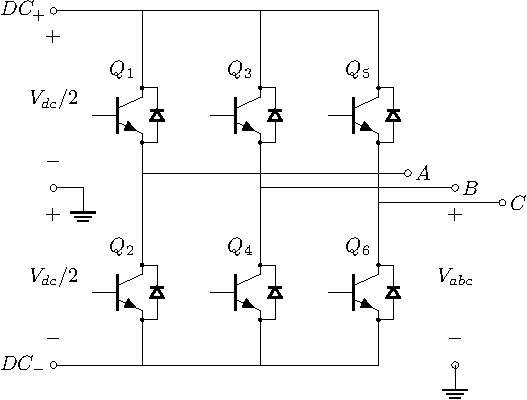
\includegraphics[width=0.9\textwidth,height=0.36\textheight,keepaspectratio]{3ph_bridge.pdf}\\[0.2em]
      {\footnotesize 6 switches\\Standard $3\phi$ VSC}
    \end{column}
  \end{columns}
  \vspace{0.4em}
  \begin{alertblock}{Modern Multilevel Topologies}
    \footnotesize
    NPC (Neutral Point Clamped), T-Type, MMC (Modular Multilevel Converter), etc. (beyond the scope of this lecture).
  \end{alertblock}
\end{frame}

% -----------------------------------------------------------------------------
% Slide 10: AC-DC VSC for Grid Applications
% -----------------------------------------------------------------------------
\begin{frame}{AC-DC VSC for Grid Applications}
  \begin{block}{Motivation}
    \begin{itemize}\small
      \item \textbf{AC:} Historically, the electricity grid was built based on AC systems.
      \item \textbf{DC:} PV panels are DC sources that are available worldwide and represent affordable renewable energy. Batteries are also DC, and many other sources traditionally based on AC are interfaced through back-to-back AC--DC--AC converters.
      \item \textbf{VSC:} Controlling power flow is easier by modulating voltage than with a current source, as the grid connection point behaves essentially as a voltage source.
    \end{itemize}
  \end{block}

  \begin{block}{What About Control?}
    \small
    All preceding classification criteria were based solely on the \textbf{power electronics topology} (hardware components through which power flows).\\
    $\rightarrow$ \textbf{How do we control these switches to manage voltage, current, and power?}
  \end{block}
\end{frame}

% =============================================================================
% SECTION 2: Grid Forming vs Grid Following
% =============================================================================
\section{Grid Forming or Grid Following?}

% -----------------------------------------------------------------------------
% Slide 12: Grid Forming (GFOR) or Grid Following (GFOL)?
% -----------------------------------------------------------------------------
\begin{frame}{Grid Forming (GFOR) vs. Grid Following (GFOL)}
  \vspace{-0.3em}
  {\small
  \begin{itemize}\setlength{\itemsep}{0pt}
    \item GFOR and GFOL are \textbf{control strategies}, not different converter topologies!
    \item The same physical converter can switch between GFOR and GFOL when appropriate.
  \end{itemize}}

  \begin{columns}[T]
    \begin{column}{0.48\textwidth}
      \centering
      \textbf{Grid Forming (GFOR)}\\
      \textit{\footnotesize «~I am forming a Voltage source~»}
      \vspace{0.2em}

      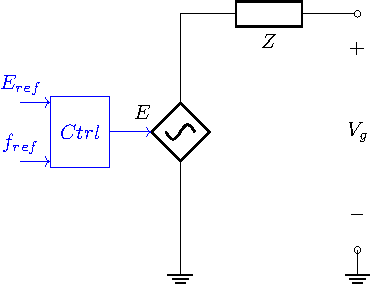
\includegraphics[width=0.72\textwidth,height=0.27\textheight,keepaspectratio]{gfor.pdf}
      \begin{itemize}\footnotesize\setlength{\itemsep}{0pt}
        \item Acts as an \textbf{ideal AC Voltage Source} ($E_{ref}, f_{ref}$)
        \item Similar in role to a synchronous generator
        \item Requires a large, controllable DC source (battery, fuel cell)
      \end{itemize}
    \end{column}

    \begin{column}{0.48\textwidth}
      \centering
      \textbf{Grid Following (GFOL)}\\
      \textit{\footnotesize «~I am following a Voltage source~»}
      \vspace{0.2em}

      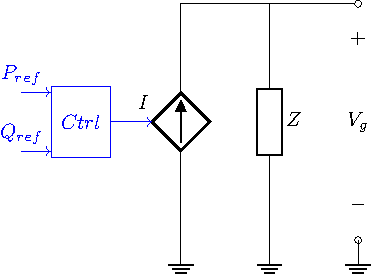
\includegraphics[width=0.72\textwidth,height=0.27\textheight,keepaspectratio]{gfol.pdf}
      \begin{itemize}\footnotesize\setlength{\itemsep}{0pt}
        \item Acts as an \textbf{AC Current Source} ($P_{ref}, Q_{ref}$)
        \item Must sense a low-distortion grid voltage ($V_g, f_g$) to synchronize
        \item Standard for renewable sources (e.g. PV with MPPT)
      \end{itemize}
    \end{column}
  \end{columns}
\end{frame}

% -----------------------------------------------------------------------------
% Slide 13: Comments on GFOR vs GFOL
% -----------------------------------------------------------------------------
\begin{frame}{Comments on GFOR vs. GFOL}
  \begin{columns}[T]
    \begin{column}{0.60\textwidth}
      \begin{itemize}\small
        \item Nowadays, almost every distributed generator (DG) like PV or wind turbines is \textbf{GFOL controlled}.
        \item As conventional synchronous machines retire ($\searrow$) and converter-interfaced DG grows ($\nearrow$), the power grid becomes \textbf{weaker} (lower physical inertia, lower short-circuit ratio).
        \item Extensive research is focused on \textbf{GFOR deployment}:
          \begin{itemize}\footnotesize
            \item Power semiconductor current limits require fast current-limiting algorithms.
            \item Basic GFOR lacks physical rotor inertia; synthetic inertia / droop control must be emulated.
          \end{itemize}
        \item Advanced concepts: \textbf{Grid Supporting Converters}, \textbf{Virtual Synchronous Machines (VSM)}, etc. [3, 4].
      \end{itemize}
    \end{column}
    \begin{column}{0.38\textwidth}
      \centering
      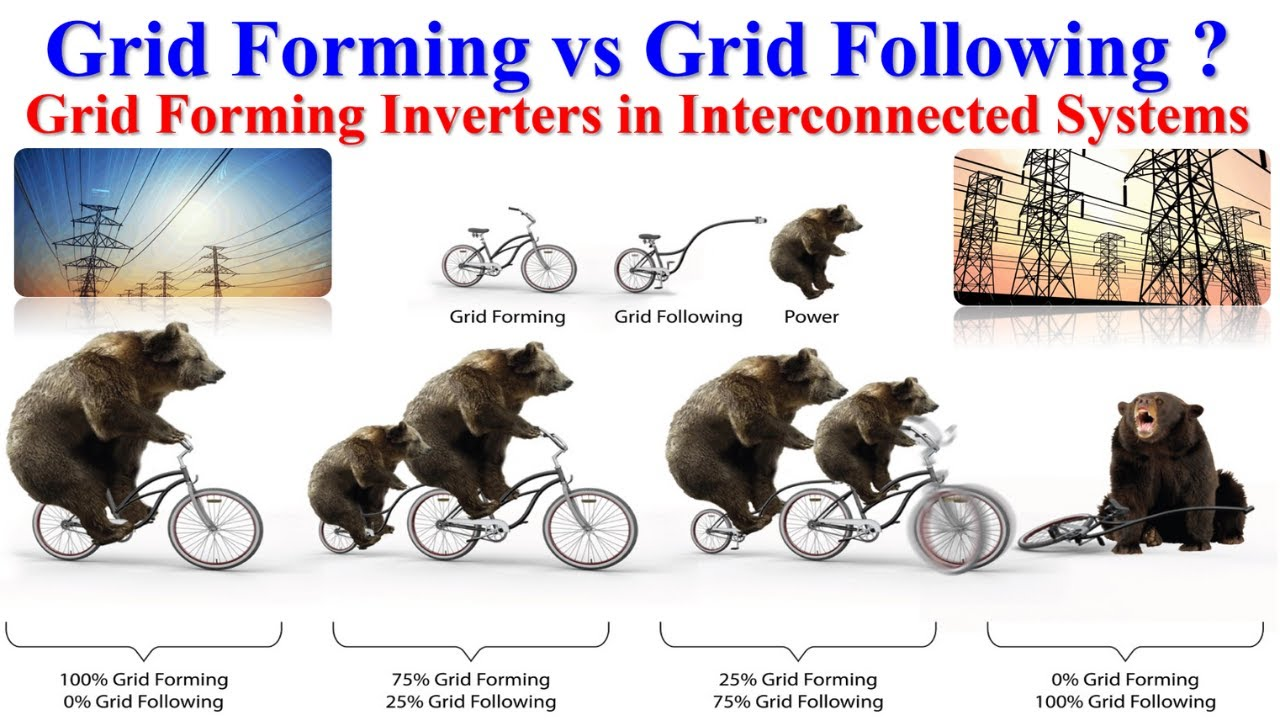
\includegraphics[width=\textwidth,height=0.65\textheight,keepaspectratio]{images/bear_meme.jpeg}
    \end{column}
  \end{columns}
\end{frame}

% -----------------------------------------------------------------------------
% Slide 14: Control Architecture
% -----------------------------------------------------------------------------
\begin{frame}{Control Architecture}
  \begin{columns}[c]
    \begin{column}{0.48\textwidth}
      \centering
      \textbf{GFOR Control Strategy}\\[0.5em]
      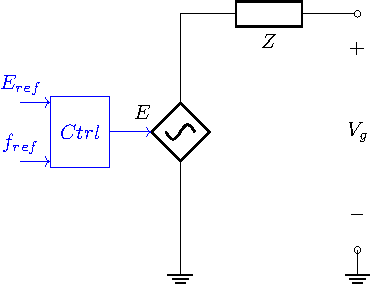
\includegraphics[width=0.78\textwidth,keepaspectratio]{gfor.pdf}
    \end{column}
    \begin{column}{0.48\textwidth}
      \centering
      \textbf{GFOL Control Strategy}\\[0.5em]
      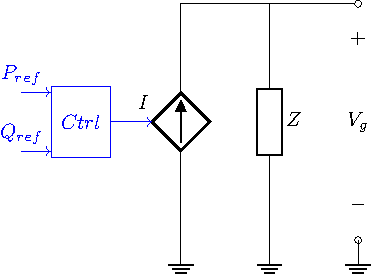
\includegraphics[width=0.78\textwidth,keepaspectratio]{gfol.pdf}
    \end{column}
  \end{columns}

  \vspace{1.2em}
  \begin{center}
    \Large \textbf{What is inside these «~Ctrl~» blocks?}
    
    \normalsize
    $\rightarrow$ Let's discover the theory and observe them with a Typhoon HIL live demo!
  \end{center}
\end{frame}

% =============================================================================
% SECTION 3: Control Design
% =============================================================================
\section{Control Design}

% -----------------------------------------------------------------------------
% Slide 16: Clarke & Park Transformation
% -----------------------------------------------------------------------------
\begin{frame}{Clarke \& Park Transformation}
  \vspace{-0.5em}
  \begin{columns}[T]
    \begin{column}{0.54\textwidth}
      \scriptsize
      \textbf{Clarke Transformation ($abc \to \alpha\beta0$):}
      \[
      T_c = \frac{2}{3}
      \begin{bmatrix}
        1 & -\frac{1}{2} & -\frac{1}{2} \\
        0 & \frac{\sqrt{3}}{2} & -\frac{\sqrt{3}}{2} \\
        \frac{1}{2} & \frac{1}{2} & \frac{1}{2}
      \end{bmatrix}
      \]
      \textbf{Rotation Matrix of angle $\omega t$:}
      \[
      R(\omega t) =
      \begin{bmatrix}
        \cos(\omega t) & \sin(\omega t) & 0 \\
        -\sin(\omega t) & \cos(\omega t) & 0 \\
        0 & 0 & 1
      \end{bmatrix}
      \]
      \textbf{Park Transformation ($T_p = R(\omega t) T_c$):}
      \[
      T_p(\omega t) = \frac{2}{3}
      \begin{bmatrix}
        \cos(\omega t) & \cos(\omega t - \frac{2\pi}{3}) & \cos(\omega t + \frac{2\pi}{3}) \\
        -\sin(\omega t) & -\sin(\omega t - \frac{2\pi}{3}) & -\sin(\omega t + \frac{2\pi}{3}) \\
        \frac{1}{2} & \frac{1}{2} & \frac{1}{2}
      \end{bmatrix}
      \]
    \end{column}
    \begin{column}{0.44\textwidth}
      \centering
      \footnotesize \textbf{Signals across coordinate frames:}\\[0.2em]
      $V_{abc}(t) \xrightarrow{\text{Clarke}} V_{\alpha\beta0}(t) \xrightarrow{\text{Rotation}} V_{dq0}(t)$\\[0.3em]
      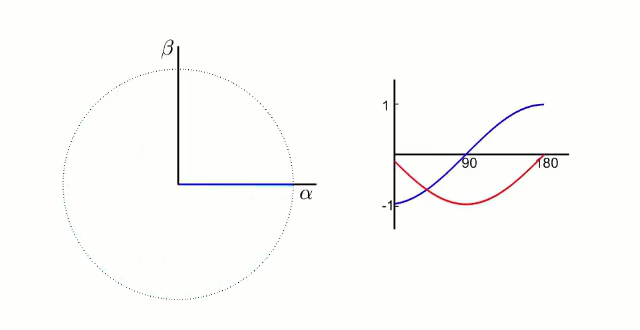
\includegraphics[width=0.82\textwidth,height=0.19\textheight,keepaspectratio]{images/waveform_abc.png}\\[0.15em]
      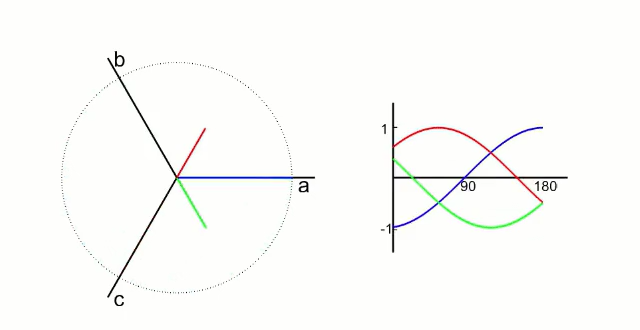
\includegraphics[width=0.82\textwidth,height=0.19\textheight,keepaspectratio]{images/waveform_ab0.png}\\[0.15em]
      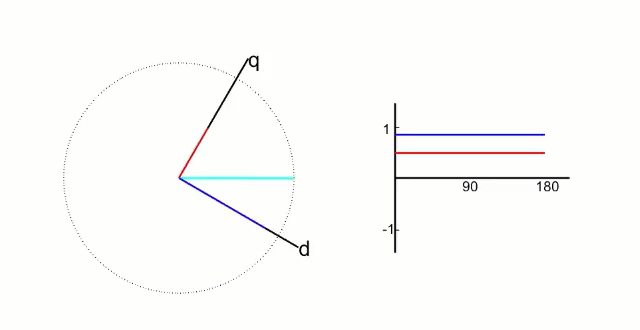
\includegraphics[width=0.82\textwidth,height=0.19\textheight,keepaspectratio]{images/waveform_dq0.png}
    \end{column}
  \end{columns}
\end{frame}

% -----------------------------------------------------------------------------
% Slide 17: Usefulness for AC Systems
% -----------------------------------------------------------------------------
\begin{frame}{Usefulness for AC Systems}
  \begin{columns}[c]
    \begin{column}{0.48\textwidth}
      \centering
      $V_{abc}(t) = \begin{bmatrix} V_a(t) \\ V_b(t) \\ V_c(t) \end{bmatrix} \xrightarrow{\quad T_p(\omega t)\quad} V_{dq0}(t) = \begin{bmatrix} V_d(t) \\ V_q(t) \\ V_0(t) \end{bmatrix}$
      
      \vspace{0.8em}
      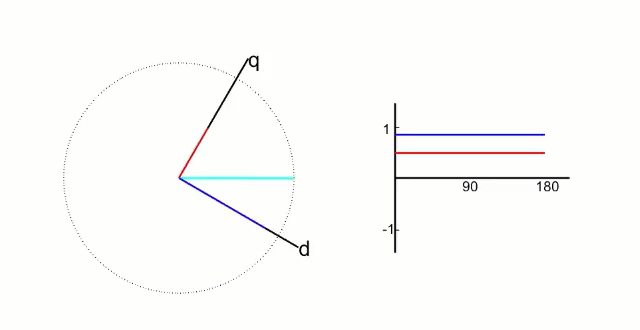
\includegraphics[width=0.88\textwidth,keepaspectratio]{images/waveform_dq0.png}
    \end{column}
    \begin{column}{0.50\textwidth}
      \begin{itemize}\small
        \item The \textbf{$dq0$ reference frame} is analogous, in terms of purpose, to the \textbf{phasor ($\underline{V}$)} concept used for sinusoidal steady-state AC circuits.
        \item It converts balanced three-phase time-varying sinusoidal signals into \textbf{constant DC quantities} in steady state.
        \item \textbf{Control theory advantage:} Time-invariant signals allow the direct application of standard linear controllers (e.g. \textbf{PI / PID controllers}) with zero steady-state error.
      \end{itemize}
    \end{column}
  \end{columns}
\end{frame}

% -----------------------------------------------------------------------------
% Slide 18: Phase-Locked Loop (PLL)
% -----------------------------------------------------------------------------
\begin{frame}{Phase-Locked Loop (PLL)}
  \vspace{-0.3em}
  {\small
  \begin{itemize}\setlength{\itemsep}{0pt}
    \item To compute the Park transform $T_p(\omega t)$, the angle $\theta(t) = \omega t$ must be known.
    \item The \textbf{Phase-Locked Loop (PLL)} tracks the grid frequency and phase angle (essential for grid-following converters).
  \end{itemize}}

  \begin{columns}[c]
    \begin{column}{0.46\textwidth}
      \textbf{Three-phase PLL operating principle:}\\[0.3em]
      \begin{enumerate}\footnotesize\setlength{\itemsep}{2pt}
        \item Apply Park transform $T_p(\hat{\theta})$ to measured grid voltages $V_{abc}$.
        \item Regulate $V_q \to 0$ using a PI controller.
        \item When $V_q = 0$, the rotating $d$-axis is aligned with the grid voltage vector.
        \item Integrator outputs tracked angle $\hat{\theta} = \omega t$.
      \end{enumerate}
    \end{column}
    \begin{column}{0.52\textwidth}
      \centering
      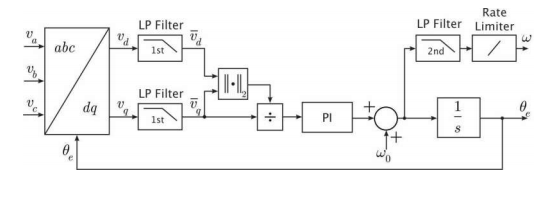
\includegraphics[width=\textwidth,keepaspectratio]{images/pll_diagram.png}
    \end{column}
  \end{columns}
\end{frame}

% -----------------------------------------------------------------------------
% Slide 19: Current Controller - Formulation
% -----------------------------------------------------------------------------
\begin{frame}{Current Controller: Governing Equations}
  \vspace{-0.3em}
  \begin{columns}[T]
    \begin{column}{0.55\textwidth}
      \begin{itemize}\small
        \item Actuators of a VSC are switching devices producing a voltage waveform $E(t)$.
        \item How do we control the current if we only command voltage?
        \item $\rightarrow$ Using \textbf{Ohm's and Faraday's laws} across the grid filter ($L, R$):
      \end{itemize}
      \[
      E(t) - V_a(t) = L \frac{dI(t)}{dt} + R I(t)
      \]
      \begin{itemize}\small
        \item Moving to the rotating $dq0$ reference frame ($V_{abc} = T_p^{-1} V_{dq0}$):
      \end{itemize}
      {\scriptsize
      \[
      T_p^{-1}(\omega t) =
      \begin{bmatrix}
        \cos(\omega t) & -\sin(\omega t) & 1 \\
        \cos(\omega t - \frac{2\pi}{3}) & -\sin(\omega t - \frac{2\pi}{3}) & 1 \\
        \cos(\omega t + \frac{2\pi}{3}) & -\sin(\omega t + \frac{2\pi}{3}) & 1
      \end{bmatrix}
      \]}
    \end{column}
    \begin{column}{0.43\textwidth}
      \centering
      \textbf{Single-Phase Equivalent AC Circuit:}\\[0.3em]
      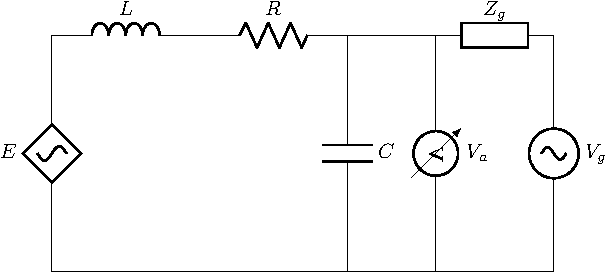
\includegraphics[width=0.95\textwidth,keepaspectratio]{vsc_ac.pdf}
    \end{column}
  \end{columns}
\end{frame}

% -----------------------------------------------------------------------------
% Slide 20: Current Controller - Decoupled dq Control
% -----------------------------------------------------------------------------
\begin{frame}{Current Controller: Decoupled $dq$ Control}
  \vspace{-0.5em}
  \begin{columns}[T]
    \begin{column}{0.62\textwidth}
      {\small Differentiating in the rotating frame yields cross-coupling terms between $d$ and $q$ axes:}
      \begin{align*}
        E_d(t) &= \color{teal}\underbrace{L \frac{dI_d(t)}{dt} + R I_d(t)}_{\text{PI output } u_d} \color{black} - \color{blue}\underbrace{L \omega I_q(t)}_{\text{cross-coupling}} \color{black} + \color{blue}\underbrace{V_d(t)}_{\text{feedforward}} \\
        E_q(t) &= \color{teal}\underbrace{L \frac{dI_q(t)}{dt} + R I_q(t)}_{\text{PI output } u_q} \color{black} + \color{blue}\underbrace{L \omega I_d(t)}_{\text{cross-coupling}} \color{black} + \color{blue}\underbrace{V_q(t)}_{\text{feedforward}}
      \end{align*}
      \begin{itemize}\footnotesize\setlength{\itemsep}{1pt}
        \item \textbf{\color{teal}PI Controller terms:} Regulate tracking errors $(I_d^* - I_d)$ and $(I_q^* - I_q)$.
        \item \textbf{\color{blue}Decoupling \& Feedforward:} Cancel cross-coupling ($\pm L\omega I$) and grid voltage disturbance ($V_{dq}$).
      \end{itemize}
    \end{column}
    \begin{column}{0.36\textwidth}
      \centering
      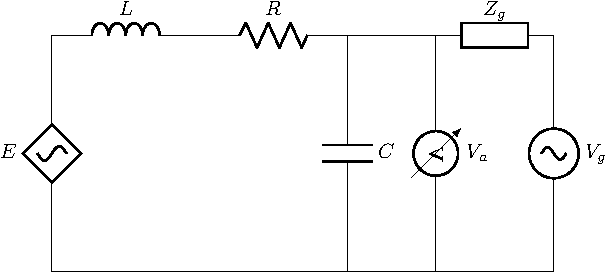
\includegraphics[width=0.95\textwidth,keepaspectratio]{vsc_ac.pdf}
    \end{column}
  \end{columns}
\end{frame}

% =============================================================================
% SECTION 4: Softstart and Islanding
% =============================================================================
\section{Softstart and Islanding}

% -----------------------------------------------------------------------------
% Slide 22: Softstart and Islanding Transients
% -----------------------------------------------------------------------------
\begin{frame}{Softstart and Islanding: Managing Transients}
  \vspace{-0.5em}
  \begin{alertblock}{Key Takeaway}
    When designing or commissioning converters, \textbf{never overlook transient electrical behaviors} before closing relays or connecting circuits!
  \end{alertblock}

  \begin{columns}[c]
    \begin{column}{0.48\textwidth}
      \centering
      \textbf{Magnetic Inrush Transient}\\[0.2em]
      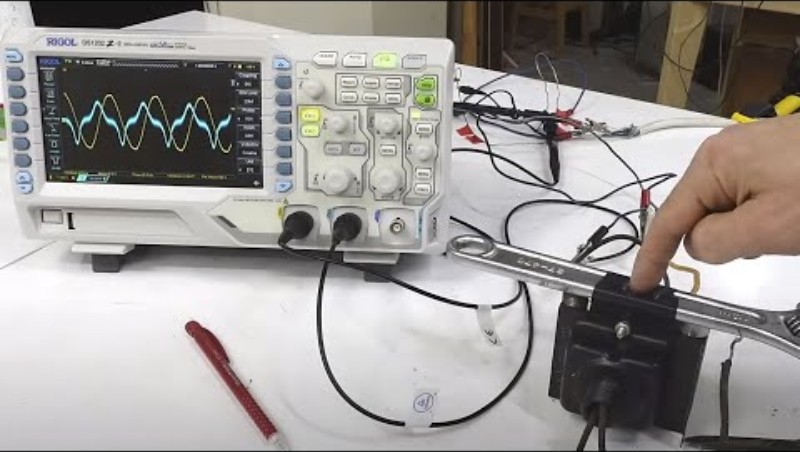
\includegraphics[width=0.95\textwidth,height=0.42\textheight,keepaspectratio]{images/magnetic_transient.jpeg}\\[0.2em]
      {\footnotesize Transformer core saturation upon energization}
    \end{column}
    \begin{column}{0.48\textwidth}
      \centering
      \textbf{Capacitive Inrush Transient}\\[0.2em]
      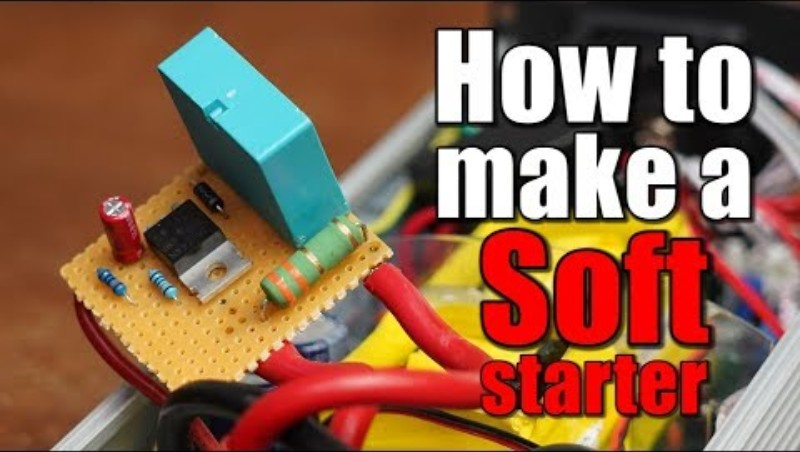
\includegraphics[width=0.95\textwidth,height=0.42\textheight,keepaspectratio]{images/capacitive_transient.jpeg}\\[0.2em]
      {\footnotesize Uncontrolled charging of DC-link capacitors}
    \end{column}
  \end{columns}
\end{frame}

% =============================================================================
% SECTION 5: Summary
% =============================================================================
\section{Summary}

% -----------------------------------------------------------------------------
% Slide 24: Key Takeaways
% -----------------------------------------------------------------------------
\begin{frame}{Key Takeaways}
  \begin{itemize}\small
    \item \textbf{VSCs} are AC/DC converters with constant DC voltage polarity, modulating the desired waveform on the AC side.
    \item To operate properly as an inverter, a VSC requires $V_{dc} \ge \max_t V_a(t)$ (for full bridge).
    \item Active power $P$ can flow from AC to DC uncontrolled via the anti-parallel body diodes if $V_{dc} \le \max_t V_a(t)$.
    \item \textbf{GFOR} acts as a \textbf{Voltage Source}; \textbf{GFOL} acts as a \textbf{Current Source}.
    \item In practice, simple open-loop GFOR exists only in islanded microgrids with ideal sources. Real grid-connected GFOR converters implement $P$ and $Q$ current limitations to protect semiconductors.
    \item A \textbf{PLL} is a dedicated closed-loop control unit that tracks the frequency and phase angle of an AC voltage signal.
  \end{itemize}
\end{frame}

% -----------------------------------------------------------------------------
% Slide 25: Summary: Grid-Connected Operation
% -----------------------------------------------------------------------------
\begin{frame}{Summary: Grid-Connected Operation}
  \framesubtitle{Room 0/64 B37 Educational Microgrid}
  \begin{center}
    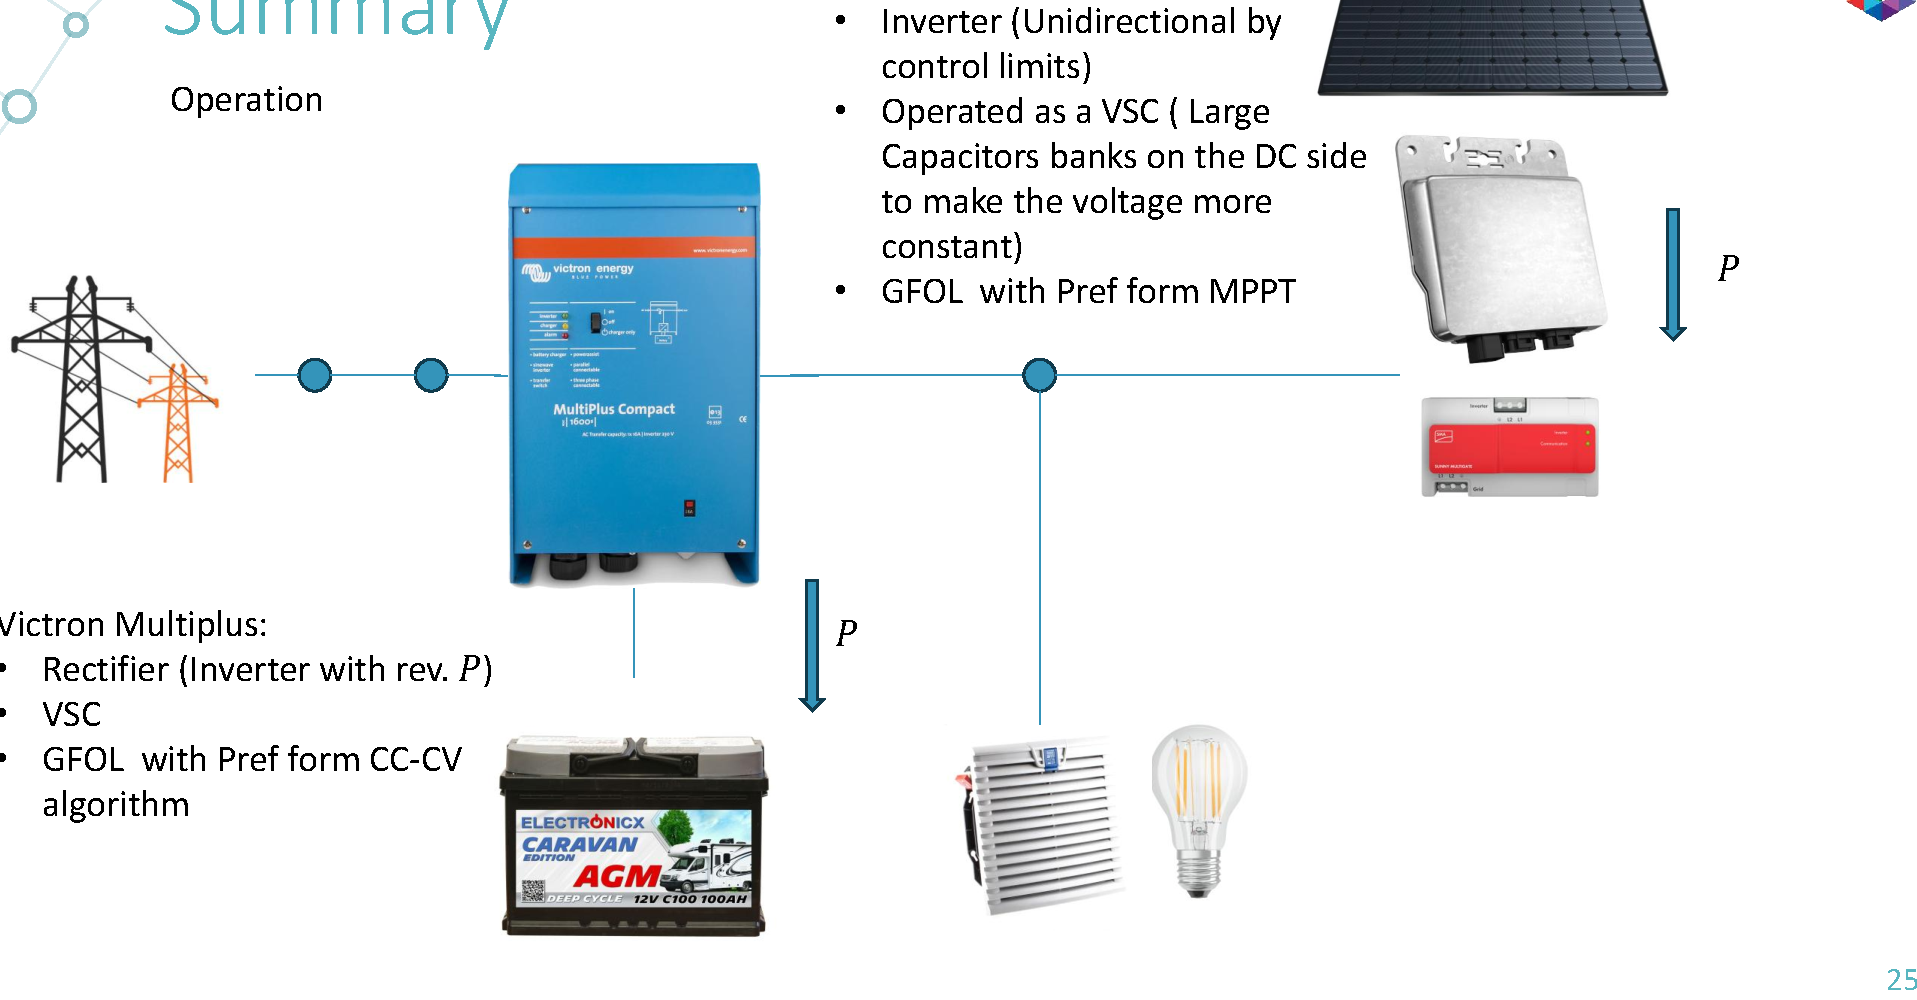
\includegraphics[width=0.90\textwidth,height=0.68\textheight,keepaspectratio]{images/operation_grid_connected.pdf}
  \end{center}
\end{frame}

% -----------------------------------------------------------------------------
% Slide 26: Summary: Islanded Microgrid Operation
% -----------------------------------------------------------------------------
\begin{frame}{Summary: Islanded Microgrid Operation}
  \framesubtitle{Room 0/64 B37 Educational Microgrid}
  \begin{center}
    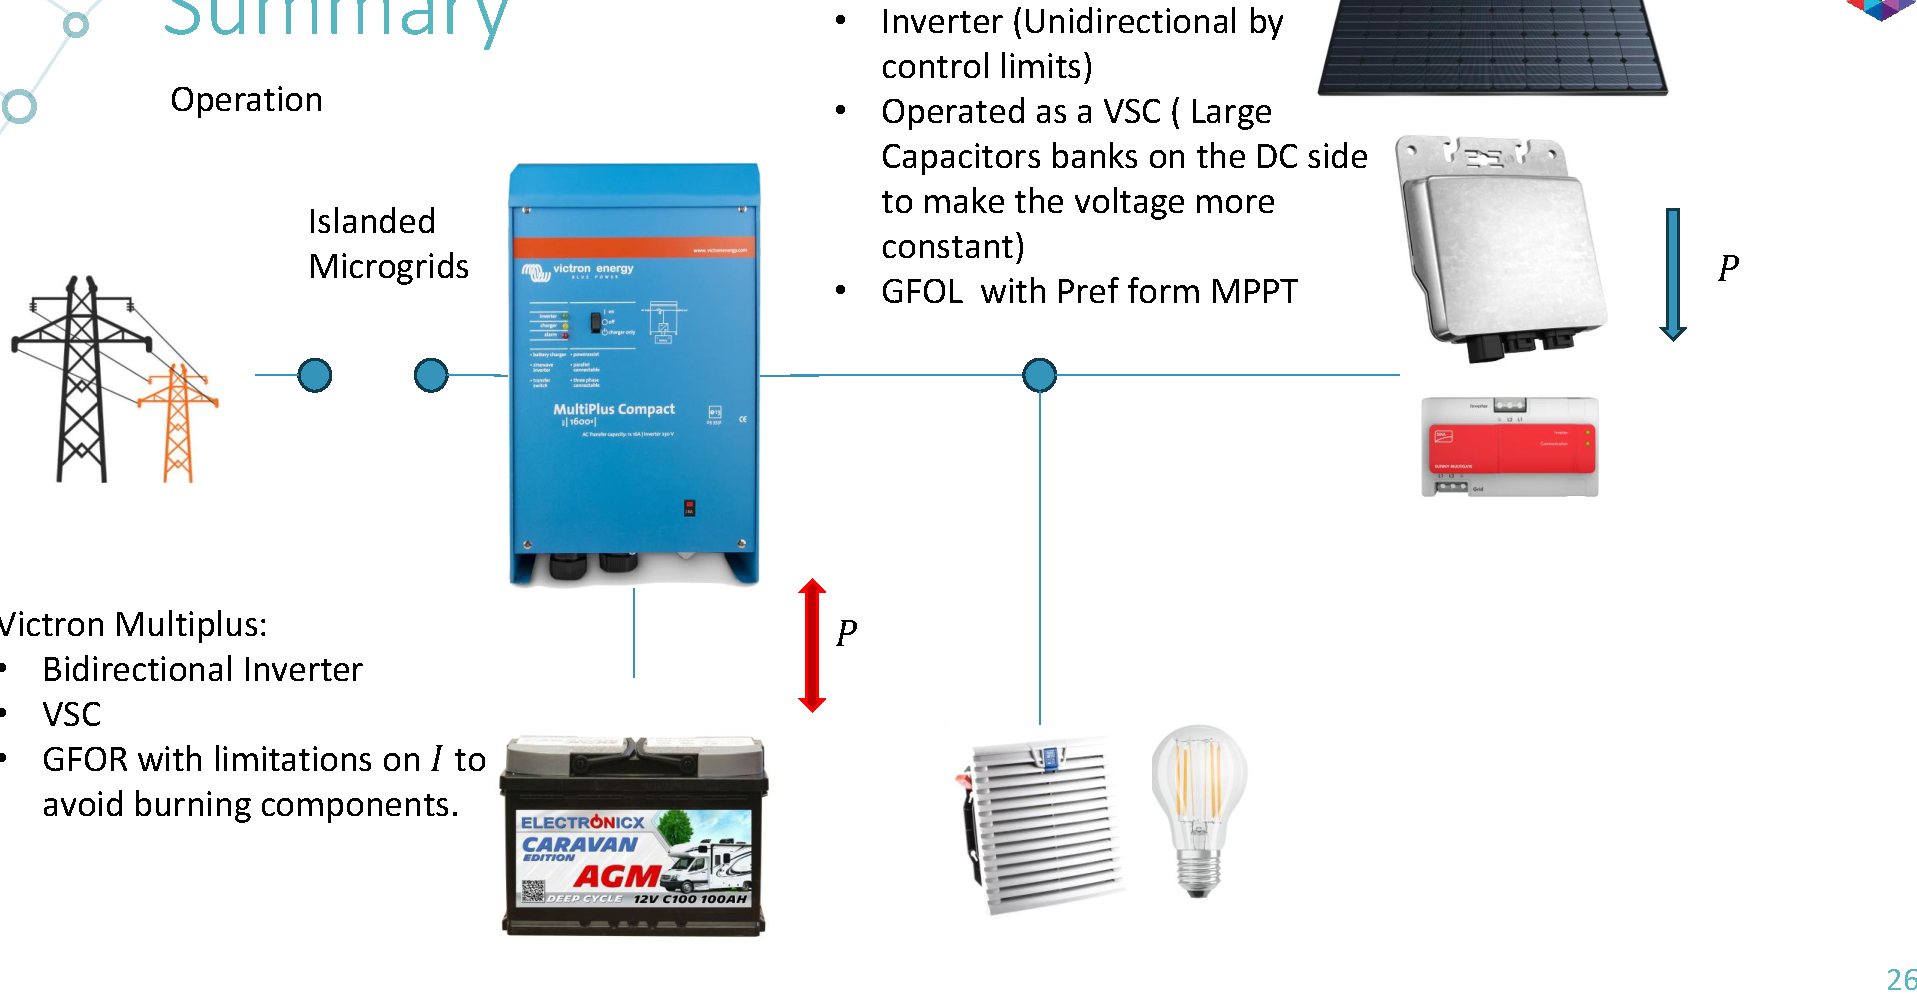
\includegraphics[width=0.90\textwidth,height=0.68\textheight,keepaspectratio]{images/operation_islanded.pdf}
  \end{center}
\end{frame}

% -----------------------------------------------------------------------------
% Slide 27: References
% -----------------------------------------------------------------------------
\begin{frame}{References}
  \footnotesize
  \begin{enumerate}
    \item Mohan, N., Undeland, T. M., \& Robbins, W. P. (1995). \emph{Power Electronics: Converters, Applications, and Design} (2nd ed.). John Wiley \& Sons.
    \item Yazdani, A., \& Iravani, R. (2010). \emph{Voltage-Sourced Converters in Power Systems: Modeling, Control, and Applications} (1st ed.). Wiley. \url{https://doi.org/10.1002/9780470551578}
    \item Rocabert, J., Luna, A., Blaabjerg, F., \& Rodríguez, P. (2012). Control of Power Converters in AC Microgrids. \emph{IEEE Transactions on Power Electronics}, 27(11), 4731--4746. \url{https://doi.org/10.1109/TPEL.2012.2199334}
    \item Zhang, H., Xiang, W., Lin, W., \& Wen, J. (2021). Grid Forming Converters in Renewable Energy Sources Dominated Power Grid: Control Strategy, Stability, Application, and Challenges. \emph{Journal of Modern Power Systems and Clean Energy}, 9(6), 1239--1256. \url{https://doi.org/10.35833/MPCE.2021.000257}
  \end{enumerate}
\end{frame}
